\documentclass{standalone}

\usepackage[english]{babel}

% to define font size

\usepackage{ulem}
\usepackage{moresize}
\usepackage{anyfontsize}

% to use colors

\usepackage[dvipsnames]{xcolor}
\usepackage{MnSymbol}

% to use tikz and its libraries

\usepackage{tikz-timing}
\usepackage{tikz}

\usetikzlibrary{backgrounds}
\usetikzlibrary{positioning, calc, arrows, shapes, automata, petri, patterns,decorations.markings}
\usetikzlibrary{decorations.pathreplacing}

% to use tikzmark, to place and refer to marks outside the current figure

\tikzset{every picture/.style={remember picture}}

% styles for transitions

\tikzset{transition/.append style={fill=black!20, thick}}
\tikzset{transition/.append style={fill=black!20, thick}}

% styles for test and inhib arcs.

\tikzstyle{test}=[pre, *-]
\tikzstyle{inhib}=[pre, o-]

\usepackage{circuitikzgit}
\ctikzset{
  logic ports=ieee,
}

% Arrow positioning in a path

\tikzset{->-/.style={decoration={
  markings,
  mark=at position #1 with {\arrow{>}}},postaction={decorate}}}

\tikzset{-<-/.style={decoration={
  markings,
  mark=at position #1 with {\arrow{<}}},postaction={decorate}}}

% shift values

\newcommand{\outportshift}{0mm}
\newcommand{\outportidpshift}{0mm}

%%%%%%%%%%%%%%%%%%%%%%%%%%%%%%%%%%%%%%%%%%%%%%%%%%
%                  BEGIN DOCUMENT                %
%%%%%%%%%%%%%%%%%%%%%%%%%%%%%%%%%%%%%%%%%%%%%%%%%%

\begin{document}

\begin{circuitikz}

  \ctikzset{multipoles/dipchip/width=2.5}
  \ctikzset{multipoles/dipchip/pin spacing=.18}

  \node (pn) {
    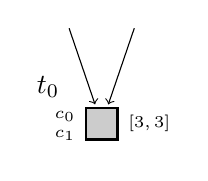
\begin{tikzpicture}

      % PLACES AND TRANSITIONS
      
      \node[transition] (t0) {};
      \node[anchor=west] at ($(t0.east)$) {\ssmall $[3,3]$};
      \node[anchor=east] at ($(t0.west)$) {\ssmall
        \begin{tabular}[h]{@{}l@{}}
          $c_0$ \\
          $c_1$ \\
        \end{tabular}
      };
      
      % LABELS

      \node[anchor=south east] (tzLabel) at ($(t0.north west)-(.2,0)$) {$t_0$};
      
      % ARCS
      
      \draw (t0) edge[pre] ($(t0.north west)-(.2,-1)$);
      \draw (t0) edge[pre] ($(t0.north east)+(.2,1)$);
      
    \end{tikzpicture}
  };
  
  % PCI idp
  
  % interface
  
  \draw       
  node [dipchip, num pins=20, hide numbers,
  no topmark, external pins width=0]
  (idp) at ($(pn.east)+(4,0)$) {};

  \node[anchor=south] at ($(idp.north)$) {$\gamma(t_0)$};
  
  \draw ($(idp.bpin 1)$)
  node [anchor=west, font=\ssmall] {\tt A}
  -- ++(-.3,0)
  node[anchor=east, font=\ssmall,xshift=\outportshift] {\tt \textcolor{blue}{3}};

  \draw ($(idp.bpin 2)$)
  node [anchor=west, font=\ssmall] {\tt B}
  -- ++(-.3,0)
  node[anchor=east, font=\ssmall,xshift=\outportshift] {\tt \textcolor{blue}{3}};
  
  \draw ($(idp.bpin 3)$)
  node (icZero) [anchor=west, font=\ssmall] {\tt ic(0)}
  -- ++(-.3,0);

  \draw ($(idp.bpin 4)$)
  node (icOne) [anchor=west, font=\ssmall] {\tt ic(1)} 
  -- ++(-.3,0);

  \draw [
  decorate, 
  decoration = {brace,
    raise=-2pt,
    amplitude=3pt,
    aspect=0.5}] ($(icZero.east)$) --  ($(icOne.east)$)
  node[anchor=west,pos=.5]{\ssmall
    \begin{tabular}[h]{@{}l}
      $=\mathtt{cn}$ \\
      $(=\vert\mathtt{conds}(t_0)\vert)$ \\
    \end{tabular}
  };

  \draw ($(idp.bpin 5)$)
  node (iavZero) [anchor=west, font=\ssmall]  {\tt iav(0)}
  -- ++(-.3,0);

  \draw ($(idp.bpin 6)$)
  node (iavOne) [anchor=west, font=\ssmall]  {\tt iav(1)}
  -- ++(-.3,0);

  \draw [
  decorate, 
  decoration = {brace,
    raise=-2pt,
    amplitude=3pt,
    aspect=0.5}] ($(iavZero.east)$) --  ($(iavOne.east)$)
  node[anchor=west,pos=.5]{\ssmall
    \begin{tabular}[h]{@{}l}
      $=\mathtt{ian}$ \\
      $(=\vert\mathtt{input}(t_0)\vert)$ \\
    \end{tabular}
  };
  
  \draw ($(idp.bpin 7)$)
  node (rtZero) [anchor=west, font=\ssmall]  {\tt rt(0)}
  -- ++(-.3,0);

  \draw ($(idp.bpin 8)$)
  node (rtOne) [anchor=west, font=\ssmall]  {\tt rt(1)}
  -- ++(-.3,0);

  \draw [
  decorate, 
  decoration = {brace,
    raise=-2pt,
    amplitude=3pt,
    aspect=0.5}] ($(rtZero.east)$) --  ($(rtOne.east)$)
  node[anchor=west,pos=.5]{\ssmall $=\mathtt{ian}$};
  
  \draw ($(idp.bpin 9)$)
  node (pahZero) [anchor=west, font=\ssmall]  {\tt pah(0)}
  -- ++(-.3,0) coordinate (idpoat0);

  \draw ($(idp.bpin 10)$)
  node (pahOne) [anchor=west, font=\ssmall]  {\tt pah(1)}
  -- ++(-.3,0);

  \draw [
  decorate, 
  decoration = {brace,
    raise=-2pt,
    amplitude=3pt,
    aspect=0.5}] ($(pahZero.east)$) -- ($(pahOne.east)$)
  node[anchor=west,pos=.5]{\ssmall $=\mathtt{ian}$};

  % Output port interface

  \draw ($(idp.bpin 15)$)
  node [anchor=east, font=\ssmall]  {\tt f}
  -- ++(.3,0);
  
  % generic map
  \node[anchor=north] at (idp.south) {\ssmall
    \begin{tabular}{@{}c@{}}
      ($\mathtt{tt}\Rightarrow\mathtt{temp\_a\_a}$),
      ($\mathtt{ian}\Rightarrow\vert{}\mathtt{input}(t_0)\vert$), \\
      ($\mathtt{cn}\Rightarrow\vert\mathtt{conds}(t_0)\vert$),
      ($\mathtt{mtc}\Rightarrow{}3$) \\
    \end{tabular}
  };

  \node at ($(pn.east)!.3!(idp.west)$) {\Huge$\rightarrow$};
  
\end{circuitikz}


\end{document}
%%% Local Variables:
%%% mode: latex
%%% TeX-master: t
%%% End:
